\chapter{Суперпространство и построение суперсимметричной динамики}

\lectureoverview{Мы заново строим суперсимметрию, начиная с наименьшей системы, в которой она может действовать: одного бозонного осциллятора и одного фермионного осциллятора с одинаковой энергией. Контраст между их уравнениями второго и первого порядка приводит к суперзарядам и их алгебре. Затем мы переинтерпретируем эту алгебру как геометрию на пространстве с обычной координатой (t) и грассмановыми координатами \(\theta,\bar\theta\). Суперполя объединяют бозоны, фермионы и вспомогательное поле в один объект; интегрирование Березина выделяет инвариантный обычный лагранжиан; ковариантные производные делают возможными ограничения, совместимые с симметрией; а киральное ограничение даёт первый важный пример. На лекции намеренно вскрываются трудности со знаками и порядком множителей в этом аппарате, а в заключение объясняется, почему сама симметрия более фундаментальна, чем перечень правил Фейнмана.}

\section{Возвращение к одномодовой системе}

Начнём снова с фермионов и бозонов в покое. Мы опускаем все пространственные координаты и все метки импульса. В данной моде квант либо присутствует, либо отсутствует, и для его описания достаточно операторов рождения и уничтожения. Обозначим бозонную моду через \(a^\dagger,a\), а фермионную — через \(c^\dagger,c\). Они удовлетворяют соотношениям
\begin{align}
[a,a^\dagger]&=1,
&
\{c,c^\dagger\}&=1,
&
c^2=(c^\dagger)^2&=0.
\end{align}
Если оба кванта имеют одинаковую энергию \(m\), то с точностью до несущественной вакуумной константы
\begin{equation}
H=m\left(a^\dagger a+c^\dagger c\right).
\label{eq:l7-one-mode-hamiltonian}
\end{equation}
Оператор числа \(a^\dagger a\) может принимать любые неотрицательные целые значения, тогда как \(c^\dagger c\) — только 0 или 1. Это и есть вся кинематика этой игрушечной модели.

Это упрощение стратегично. Мы хотим понять операцию, которая уничтожает бозон и создаёт фермион, или делает обратное, не изменяя энергии. Однако прежде чем строить эту операцию, переведём ту же систему с операторного языка на язык лагранжиана.

\section{Бозонный осциллятор}

Для бозона введём вещественную координату \(\phi(t)\). При отсутствии пространственной зависимости свободное скалярное поле превращается в обычный гармонический осциллятор. Первое выражение, написанное на доске, было
\[
\frac{1}{2}\dot\phi^{,2}+\frac{1}{2}m^2\phi^2.
\]
Это выражение есть сумма кинетической и потенциальной энергий, а не лагранжиан. На лекции знак сразу же исправляется:
\begin{equation}
L_B=\frac{1}{2}\dot\phi^{,2}-\frac{1}{2}m^2\phi^2.
\label{eq:l7-boson-lagrangian}
\end{equation}

\begin{figure}[H]
\centering
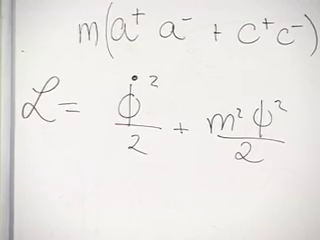
\includegraphics[width=0.62\textwidth]{lecture_07_figure_02.png}
\lectureframe{00:03:25.431}
\caption{Одномодовый гамильтониан над бозонным лагранжианом. На кадре сохранён исходный знак плюс до устного исправления на \(T-V\).}
\end{figure}

\begin{classroomqa}
\audiencequestion{Что не так со знаком в выписанном лагранжиане осциллятора? \lecturetimestamp{00:04:00}}
\lecturerresponse{Энергия равна \(T+V\), а лагранжиан — \(T-V\). Поэтому потенциальный член должен входить с минусом. Исправление меняет уравнение так, что вместо экспоненциального поведения получаются ожидаемые гармонические колебания.}
\end{classroomqa}

Действительно, уравнение Эйлера--Лагранжа даёт
\begin{align}
\frac{d}{dt}\frac{\partial L_B}{\partial\dot\phi}
&=\frac{\partial L_B}{\partial\phi},\\
\ddot\phi&=-m^2\phi,
\end{align}
или
\begin{equation}
\ddot\phi+m^2\phi=0.
\label{eq:l7-boson-eom}
\end{equation}
Его частота равна \(m\), а не \(m^2\). Квантование этого осциллятора воспроизводит ту же лестницу состояний, которая описывается \(a^\dagger\) и \(a\) в уравнении~\eqref{eq:l7-one-mode-hamiltonian}.

\section{Почему фермионное действие имеет первый порядок}

Фермионный лагранжиан выглядит проще, потому что содержит только одну производную по времени. Причина уже видна в намеренно наивной пробе. Для обычной коммутирующей переменной
\begin{equation}
L_{\mathrm{trial}}=\phi\dot\phi
=\frac{1}{2}\frac{d}{dt}\phi^2.
\end{equation}
это полная производная. Соответствующее уравнение Эйлера--Лагранжа утверждает лишь \(\dot\phi=\dot\phi\), так что допустим любой дифференцируемый путь. Вычитание полной производной из действия меняет граничные данные, но не внутреннее уравнение движения.

Теперь переименуем переменную в \(\psi\) и объявим её грассманово нечётной. И \(\psi\), и \(\dot\psi\) антикоммутируют. При фиксированном выборе левой вариации перестановка нечётных множителей вносит минус, так что та же формальная проба даёт
\begin{equation}
\frac{d}{dt}\frac{\partial L_{\mathrm{trial}}}{\partial\dot\psi}
=\dot\psi,
\qquad
\frac{\partial L_{\mathrm{trial}}}{\partial\psi}
=-\dot\psi.
\end{equation}
Следовательно, уравнение имеет вид
\begin{equation}
\dot\psi=-\dot\psi
\quad\Longrightarrow\quad
\dot\psi=0.
\label{eq:l7-constant-fermion}
\end{equation}
Выражение, которое для коммутирующей координаты было тавтологией, для антикоммутирующей приобрело динамическое содержание. Для осциллятора это условие слишком жёстко, поскольку допускает только константу, но именно эта подсказка нам и нужна.

\begin{classroomqa}
\audiencequestion{Неужели решение просто в том, что \(\psi\) — константа? \lecturetimestamp{00:13:57}}
\lecturerresponse{Да. Уравнение~\eqref{eq:l7-constant-fermion} — это настоящее дифференциальное уравнение первого порядка, и его решением служит произвольная грассманнозначная константа. Массовый член превратит это статическое решение в осциллирующее.}
\end{classroomqa}

Очевидная попытка, \(m\psi^2\), не проходит, потому что \(\psi^2=0\). Нужны две вещественные нечётные переменные \(\psi_1,\psi_2\), или, что эквивалентно, одна комплексная переменная и её сопряжённая. На лекции на доске разбирается форма с двумя вещественными переменными, с многократной проверкой знаков и множителей 2. При обычной нормировке комплексная форма имеет вид
\begin{equation}
L_F=\frac{i}{2}
\left(\bar\psi\dot\psi-\dot{\bar\psi}\psi\right)
-m\bar\psi\psi.
\label{eq:l7-fermion-lagrangian}
\end{equation}
С точностью до полной производной это \(i\bar\psi\dot\psi-m\bar\psi\psi\). Варьирование по \(\bar\psi\) даёт
\begin{equation}
i\dot\psi=m\psi,
\qquad
\psi(t)=\psi(0)e^{-imt}.
\label{eq:l7-fermion-eom}
\end{equation}
Сопряжённое уравнение имеет противоположную фазу. Таким образом, фермионная мода осциллирует с энергией \(m\), как и бозонная, хотя её уравнение первого, а не второго порядка.

\editorialnote{Формула~\eqref{eq:l7-fermion-lagrangian} фиксирует один стандартный порядок множителей и нормировку для пробного расчёта с двумя вещественными переменными. На самой лекции вводится множитель \(i\), подправляется множитель 2, и знак у одной вещественной компоненты остаётся неуточнённым. Эти изменения не меняют главного вывода: кинетический член фермиона имеет первый порядок, масса входит линейно, а комплексный фермион даёт ненулевую билинейную комбинацию.}

Это нульмерная тень знакомого релятивистского контраста. Уравнение Клейна--Гордона имеет второй порядок по времени, тогда как уравнение Дирака — первый. При опущенной пространственной зависимости бозон — это один гармонический осциллятор, а фермион — один комплексный грассмановский осциллятор.

\begin{classroomqa}
\audiencequestion{Имеет ли значение порядок, в котором записываются \(\psi\), \(\dot\psi\) и их сопряжённые? \lecturetimestamp{00:18:58}}
\lecturerresponse{Промежуточные формулы действительно зависят от порядка, потому что нечётные множители антикоммутируют. Физическая теория не зависит от произвольного предпочтения в записи, если повсюду последовательно использовать одну и ту же конвенцию для левой или правой вариации, сопряжения и интегрирования. Перестановка нечётной пары меняет знак, и тогда его нужно везде последовательно изменить.}
\end{classroomqa}

Объединяя уравнения~\eqref{eq:l7-boson-lagrangian} и \eqref{eq:l7-fermion-lagrangian}, мы получаем лагранжево описание той же пары, которая представлена уравнением~\eqref{eq:l7-one-mode-hamiltonian}. Теперь мы готовы выделить симметрию между ними.

\section{Суперзаряды и их алгебра}

Оператор, который уничтожает фермион и создаёт бозон, имеет вид
\begin{equation}
Q^\dagger=\sqrt{2m}\,a^\dagger c,
\end{equation}
тогда как его сопряжённый уничтожает бозон и создаёт фермион,
\begin{equation}
Q=\sqrt{2m}\,a c^\dagger.
\end{equation}
Нормировка выбрана так, чтобы алгебра принимала стандартный вид. Используя \(cc^\dagger=1-c^\dagger c\), \(aa^\dagger=a^\dagger a+1\) и тот факт, что бозонные и фермионные операторы коммутируют друг с другом,
\begin{align}
\{Q,Q^\dagger\}
&=2m\left(ac^\dagger a^\dagger c+a^\dagger c a c^\dagger\right)\notag\\
&=2m\left[(a^\dagger a+1)c^\dagger c
+a^\dagger a(1-c^\dagger c)\right]\notag\\
&=2m\left(a^\dagger a+c^\dagger c\right)=2H.
\label{eq:l7-superalgebra}
\end{align}
Бозонные операторы можно переносить через фермионные. Та же нильпотентность, которая ограничивает заполнение фермионной моды, даёт
\begin{equation}
Q^2=(Q^\dagger)^2=0.
\end{equation}
Наконец,
\begin{equation}
[H,Q]=[H,Q^\dagger]=0.
\label{eq:l7-conserved-supercharges}
\end{equation}
Каждый суперзаряд изменяет число бозонов и число фермионов в противоположных направлениях, так что при равных частотах два изменения энергии компенсируют друг друга.

\begin{classroomqa}
\audiencequestion{Чему равно \([H,Q]\)? Пропорционален ли ответ \(Q\)? \lecturetimestamp{00:25:10}}
\lecturerresponse{Нет. Ответ равен нулю. Отдельный оператор рождения или уничтожения при коммутировании с \(H\) получил бы множитель, равный своей энергии, но бозонный и фермионный вклады в \(Q\) сокращаются. Именно это сокращение и выражает условие равенства энергий.}
\end{classroomqa}

\begin{classroomqa}
\audiencequestion{Разве этот коммутатор уже не был написан на доске? \lecturetimestamp{00:25:45}}
\lecturerresponse{Был. Повторное получение полезно, потому что заставляет нас не просто переписать это соотношение, а интерпретировать его: коммутирование с гамильтонианом означает, что преобразование является симметрией и что его генератор сохраняется.}
\end{classroomqa}

Слово \emph{заряд} отражает этот закон сохранения. Однако не следует рассматривать \(Q\) как обычное совместно измеримое число, приписанное состоянию. Он грассманово нечётен, нильпотентен и переводит бозонное состояние в фермионное. Содержательное утверждение состоит в том, что это сохраняющийся генератор, действующий внутри вырожденных супермультиплетов.
\editorialnote{Эта формулировка уточняет использованную в аудитории аналогию с маркировкой состояний по энергии или электрическому заряду. Отдельные неэрмитовы нечётные суперзаряды не являются обычными наблюдаемыми с числовыми квантовыми метками. Их сохраняющееся действие и представление полной супералгебры дают правильную классификацию.}

\section{Генераторы как производные}

Алгебра компактна, но сама по себе она не говорит нам, как строить теории с взаимодействием. Следующий шаг — геометрический. Знакомые генераторы симметрий уже действуют как дифференциальные операторы. В соглашении, принятом на лекции,
\begin{equation}
H=i\frac{\partial}{\partial t},
\qquad
P=-i\frac{\partial}{\partial x}.
\end{equation}

\begin{figure}[H]
\centering
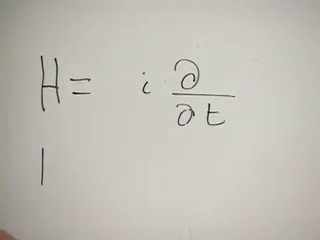
\includegraphics[width=0.50\textwidth]{lecture_07_figure_03.png}
\lectureframe{00:28:12.720}
\caption{Гамильтониан, представленный как генератор временных трансляций.}
\end{figure}

Угловой момент аналогично представляет собой координату, умноженную на производную. Если суперзаряды являются нечётными генераторами, естественно спросить, можно ли представить их производными по нечётным координатам. Поэтому мы расширяем ось времени до суперпространства
\begin{equation}
(t,\theta,\bar\theta),
\qquad
\theta^2=\bar\theta^2=0,
\qquad
\theta\bar\theta=-\bar\theta\theta.
\end{equation}
Поля на этом пространстве зависят от обычного времени и сопряжённой пары грассмановых координат.

Лекция намеренно показывает, насколько коварны знаки. Знак, возникающий при комплексном сопряжении, знак, возникающий при перестановке нечётного параметра, и знак, связанный с выбором левых, а не правых производных, соответствуют разным операциям. Вместо того чтобы сохранять взаимно несовместимые этапы выкладок на доске, мы теперь фиксируем одно соглашение: все нечётные производные являются левыми, и
\begin{equation}
q=\partial_\theta+i\bar\theta\partial_t,
\qquad
\bar q=\partial_{\bar\theta}+i\theta\partial_t.
\label{eq:l7-differential-supercharges}
\end{equation}
Тогда
\begin{equation}
q^2=\bar q^{,2}=0,
\qquad
\{q,\bar q\}=2i\partial_t=2H.
\label{eq:l7-differential-algebra}
\end{equation}
Коэффициент 2 возникает из двух перекрёстных членов: \(\{\partial_\theta,\theta\}=1\) и \(\{\partial_{\bar\theta},\bar\theta\}=1\). Если бы генераторы содержали только \(\partial_\theta\) и \(\partial_{\bar\theta}\), их антикоммутатор обращался бы в нуль и не мог бы воспроизвести гамильтониан.

\begin{classroomqa}
\audiencequestion{Должны ли два члена с производной по времени в \(q\) и \(\bar q\) иметь один и тот же знак? \lecturetimestamp{00:31:01}}
\lecturerresponse{Их нужно выбирать согласованно, так чтобы смешанный антикоммутатор был \(2H\). Можно использовать либо соглашение с общим плюсом, либо его согласованно сопряжённую альтернативу. Относительные знаки определяются вычислением, а не зрительной интуицией относительно символа \(i\).}
\end{classroomqa}

Аудитория снова и снова проверяет знаки, и трудность превращается в шутку: кажется, будто по дороге на работу знаки успевают измениться. Шутка уместна. Если антикоммутировать грассманов параметр с координатой, знак может измениться, даже когда никакое физическое соглашение не менялось. Уравнение~\eqref{eq:l7-differential-supercharges} служит фиксированной точкой отсчёта для всего последующего.

\subsection{Суперсимметрия как сдвиг координат}

Пусть \(\xi,\bar\xi\) — бесконечно малые нечётные параметры. Действие на суперполе посредством
\begin{equation}
\delta_\xi=\xi q+\bar\xi\bar q
\end{equation}
эквивалентно в приведённом выше соглашении бесконечно малому преобразованию координат
\begin{align}
\theta&\longrightarrow\theta+\xi,\\
\bar\theta&\longrightarrow\bar\theta+\bar\xi,\\
t&\longrightarrow t+i\left(\xi\bar\theta+\bar\xi\theta\right).
\label{eq:l7-coordinate-shift}
\end{align}
Поэтому изменение скалярного суперполя равно
\begin{equation}
\delta_\xi\Phi
=\left(\xi\partial_\theta+\bar\xi\partial_{\bar\theta}
+i\xi\bar\theta\partial_t+i\bar\xi\theta\partial_t\right)\Phi
=\left(\xi q+\bar\xi\bar q\right)\Phi.
\end{equation}
В этом состоит геометрическое содержание суперсимметрии. Это сдвиг по нечётным направлениям, связанный со сдвигом по обычному времени. Два нечётных сдвига замыкаются на сдвиг по времени в силу уравнения~\eqref{eq:l7-differential-algebra}.

\begin{classroomqa}
\audiencequestion{Может ли спорный минус означать движение назад во времени? \lecturetimestamp{00:58:13}}
\lecturerresponse{Иное соглашение о знаках может обратить показанный бесконечно малый сдвиг по времени, но никакой отдельный физический процесс обратного хода времени при этом не вводится. Важно то, что преобразование координат и дифференциальные генераторы подчиняются одной и той же алгебре.}
\end{classroomqa}

\begin{classroomqa}
\audiencequestion{Имеет ли это расширенное время физическую реализацию, или это лишь формальное средство учёта? \lecturetimestamp{00:58:23}}
\lecturerresponse{В одном полезном смысле это действительно средство учёта: оно упаковывает алгебру в геометрию. Но такая упаковка становится физически ценной, когда вводятся взаимодействия. Суперпространство даёт систематическое исчисление для построения лагранжианов, сохраняющих бозон--фермионную симметрию на каждом шаге, точно так же, как тензорное исчисление помогает нам строить скаляры Лоренца.}
\end{classroomqa}

\section{Суперполя и вспомогательная компонента}

Поскольку нечётных координат всего две, разложение чётного суперполя обрывается:
\begin{equation}
\Phi(t,\theta,\bar\theta)
=\phi(t)+\bar\theta\psi(t)+\bar\psi(t)\theta
+D(t)\bar\theta\theta.
\label{eq:l7-superfield}
\end{equation}
Коэффициенты при чётных мономах, \(\phi\) и \(D\), являются бозонными; коэффициенты при нечётных мономах, \(\psi\) и \(\bar\psi\), являются фермионными. Никакой член с \(\theta^2\), \(\bar\theta^2\) или более высокой степенью не остаётся. Зависимость от времени мы не раскладываем, потому что обычный ряд Тейлора по \(t\) не обрывался бы и здесь не служил бы никакой цели.

\begin{classroomqa}
\audiencequestion{Что представляет собой компонента \(D(t)\) в старшем члене? \lecturetimestamp{00:41:46}}
\lecturerresponse{На этом этапе это просто последний бозонный коэффициент в конечном разложении. В компонентном действии у него обычно нет кинетического члена, и он устраняется алгебраическим уравнением движения, поэтому его называют вспомогательным полем. Лектор шутливо предлагает ``D для dummy,'' что передаёт его нединамическую роль, не являясь при этом историческим определением.}
\end{classroomqa}

Суперполе — это один объект, тогда как \(\phi,\psi,\bar\psi,D\) — его компоненты. Преобразование суперсимметрии перемешивает их. Поэтому бозон и фермион связаны примерно в том же структурном смысле, в каком \(x\)- и \(y\)-компоненты вектора связаны поворотом, хотя грассмановы направления нельзя изобразить как обычные оси.

\section{Супердействие и старшая компонента}

Чтобы получить уравнения движения, нам нужно действие. В обычной теории поля строят скалярный лагранжиан и интегрируют его по пространству-времени. Здесь аналогичное выражение имеет вид
\begin{equation}
S=\int dt\,d\theta\,d\bar\theta\;\Lambda
\bigl(\Phi,\text{ superspace derivatives of }\Phi\bigr),
\label{eq:l7-superaction}
\end{equation}
где \(\Lambda\) — чётное суперполе. Интегрирование Березина алгебраично. Мы выбираем
\begin{equation}
\int d\theta\,d\bar\theta\;\bar\theta\theta=1.
\end{equation}
Следовательно, если
\begin{equation}
\Lambda=A+\bar\theta B+\bar B\theta+C\bar\theta\theta,
\end{equation}
то
\begin{equation}
\int d\theta\,d\bar\theta\;\Lambda=C.
\label{eq:l7-top-component}
\end{equation}
Интеграл по нечётным координатам выделяет старшую компоненту, оставляя обычный лагранжиан, который затем интегрируется по времени.

Почему результат инвариантен? Вариация суперсимметрии сдвигает переменные интегрирования. Вариация старшей компоненты есть обычная полная производная по времени, тогда как полные производные по нечётным координатам исчезают при интегрировании Березина. При подходящих граничных условиях действие не изменяется. Это суперпространственный аналог построения скаляра Лоренца перед его интегрированием по пространству-времени.

\section{Умножение суперполей}

Самый простой способ получить новое суперполе из старого — умножить его само на себя. Исходя из уравнения~\eqref{eq:l7-superfield}, каждый член, содержащий \(\theta^2\) или \(\bar\theta^2\), обращается в нуль. Сохраняя порядок \(\bar\theta\theta\) и записывая компоненты с чертой слева, получаем
\begin{align}
\Phi^2
={}&\phi^2
+2\phi\bar\theta\psi
+2\phi\bar\psi\theta\notag\\
&+\left(2\phi D-2\bar\psi\psi\right)\bar\theta\theta.
\label{eq:l7-superfield-square}
\end{align}

\begin{figure}[H]
\centering
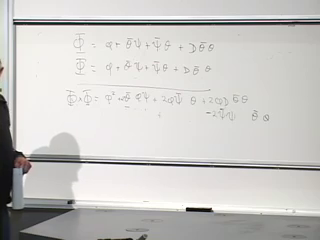
\includegraphics[width=0.82\textwidth]{lecture_07_figure_05.png}
\lectureframe{01:07:57.844}
\caption{Покомпонентное произведение суперполя и сбор всех его членов с \(\bar\theta\theta\).}
\end{figure}

Два члена \(\phi D\) и \(D\phi\) складываются, потому что оба поля чётные. Два перекрёстных фермионных члена тоже складываются после того, как каждый из них переставлен, но их общий знак отрицателен:
\begin{equation}
(\bar\theta\psi)(\bar\psi\theta)
+(\bar\psi\theta)(\bar\theta\psi)
=-2\bar\psi\psi\,\bar\theta\theta.
\end{equation}
Интегрируя квадрат по нечётным координатам, получаем
\begin{equation}
\int d\theta\,d\bar\theta\;\Phi^2
=2\phi D-2\bar\psi\psi.
\end{equation}
Этот член суперсимметричен по построению, но это ещё не кинетический лагранжиан. Он не содержит производных по времени.

Затем на доске в качестве упражнений предлагаются \(\Phi^3\), \(\Phi^4\) и \(\Phi^n\). Есть компактное правило. Для любой обычной функции \(W\),
\begin{equation}
\left.W(\Phi)\right|_{\bar\theta\theta}
=W'(\phi)D-W''(\phi)\bar\psi\psi.
\label{eq:l7-function-top-component}
\end{equation}
Для \(W(\phi)=\phi^2\) это воспроизводит уравнение~\eqref{eq:l7-superfield-square}; для \(W(\phi)=\phi^n\) получается
\begin{equation}
\left.\Phi^n\right|_{\bar\theta\theta}
=n\phi^{n-1}D-n(n-1)\phi^{n-2}\bar\psi\psi.
\end{equation}
\editorialnote{На лекции \(n\)-я степень предлагается как упражнение и перечисляются ожидаемые типы членов. Уравнение~\eqref{eq:l7-function-top-component} даёт полное правило в соглашении о фиксированном порядке.}

На этом месте лектор спрашивает, устала ли аудитория. Аудитория отвечает, что нет; он отвечает, что устал он. Этот обмен репликами — не просто комическая передышка. Степени суперполей просты, потому что разложение обрывается, но именно на производных и ограничениях учёт знаков становится по-настоящему трудным.

\section{Какие производные совместимы с суперсимметрией?}

Прежде чем переходить к следующему рассуждению на доске, нужно внести одну поправку. Обычная производная по времени безобидна:
\begin{equation}
[\partial_t,q]=[\partial_t,\bar q]=0.
\end{equation}
Следовательно, \(\partial_t\Phi\) преобразуется как суперполе всякий раз, когда так преобразуется \(\Phi\). Тонкость связана с самими нечётными производными \(\partial_\theta\Phi\) и \(\partial_{\bar\theta}\Phi\), потому что они не антикоммутируют с обоими суперзарядами. Для ограничений и для явно суперсимметричных компонентных построений нам нужны модифицированные нечётные производные.
\editorialnote{Устное утверждение о том, что дифференцирование по времени не даёт другого суперполя, неверно в используемом здесь соглашении. Поскольку \(\partial_t\) коммутирует с обоими суперзарядами, она ковариантна. Последующее построение модифицированных нечётных производных всё равно необходимо и составляет подлинную математическую суть лекции.}

\subsection{Аналогия с ``волшебным полем''}

Лекция мотивирует критерий на примере обычных поворотов. Пусть \(f(x,y)\) удовлетворяет условию
\begin{equation}
\partial_y f=0.
\label{eq:l7-magic-constraint}
\end{equation}
Назовём такую функцию ``волшебным полем''. Она зависит от \(x\), но не от \(y\). Сохраняется ли класс волшебных полей при поворотах? Для
\begin{equation}
L_z=-i\left(x\partial_y-y\partial_x\right),
\end{equation}
находим
\begin{equation}
[\partial_y,L_z]=i\partial_x\neq0.
\end{equation}
Следовательно, \(L_z f\), вообще говоря, приобретает зависимость от \(y\), даже когда \(f\) изначально удовлетворяет уравнению~\eqref{eq:l7-magic-constraint}. Это ограничение не инвариантно относительно поворотов.

Общий вывод прост. Если поле удовлетворяет \(C\Phi=0\) и симметрия порождается оператором \(G\), то преобразованное поле остаётся удовлетворяющим ограничению, когда градуированный коммутатор \(C\) и \(G\) равен нулю. Для двух нечётных операторов градуированный коммутатор есть антикоммутатор.

\begin{classroomqa}
\audiencequestion{Когда ограничение на поле совместимо с симметрией? \lecturetimestamp{01:17:56}}
\lecturerresponse{Когда оператор ограничения градуированно коммутирует с генераторами симметрии. Тогда \(C(G\Phi)\) можно перенести через \(G\) и свести к \(G(C\Phi)=0\). Пример с поворотом не работает, потому что \(\partial_y\) не коммутирует с генератором вращения.}
\end{classroomqa}

\subsection{Ковариантные нечётные производные}

Зафиксировав суперзаряды по уравнению ~\eqref{eq:l7-differential-supercharges}, определим
\begin{equation}
\mathcal D=\partial_\theta-i\bar\theta\partial_t,
\qquad
\bar{\mathcal D}=\partial_{\bar\theta}-i\theta\partial_t.
\label{eq:l7-covariant-derivatives}
\end{equation}
Единственное изменение — знак при члене с производной по времени. Прямое вычисление даёт
\begin{align}
\{\mathcal D,q\}
&=\{\mathcal D,\bar q\}
=\{\bar{\mathcal D},q\}
=\{\bar{\mathcal D},\bar q\}=0,\\
\{\mathcal D,\bar{\mathcal D}\}&=-2i\partial_t.
\label{eq:l7-covariant-algebra}
\end{align}
Два потенциально ненулевых перекрёстных члена сокращаются. Это нечётный аналог ковариантной производной: он дифференцирует, сохраняя закон преобразования.

В лекции обозначение \(D\) используется и для вспомогательной компоненты, и для этой производной. Для компоненты мы сохраняем \(D(t)\), а для оператора используем каллиграфическое \(\mathcal D\).

\section{Хиральное ограничение}

Теперь можно наложить нетривиальное ограничение, которое сохраняется при суперсимметрии:
\begin{equation}
\bar{\mathcal D}\Phi=0.
\label{eq:l7-chiral-constraint}
\end{equation}
Такое поле называется хиральным. Если до суперсимметричного преобразования оно хирально, то
\begin{equation}
\bar{\mathcal D}(q\Phi)
=-q(\bar{\mathcal D}\Phi)=0,
\qquad
\bar{\mathcal D}(\bar q\Phi)
=-\bar q(\bar{\mathcal D}\Phi)=0.
\end{equation}
Тем самым всё преобразованное суперполе остаётся внутри этого ограниченного класса. В отличие от условия магического поля, хиральность совместима с симметрией.

Чтобы решить это ограничение, введём сдвинутую временную координату
\begin{equation}
\tau=t+i\bar\theta\theta.
\label{eq:l7-chiral-time}
\end{equation}
Поскольку мы используем левые производные,
\begin{equation}
\partial_{\bar\theta}\tau=i\theta,
\end{equation}
а значит,
\begin{equation}
\bar{\mathcal D}F(\tau,\theta)
=\left(\partial_{\bar\theta}-i\theta\partial_t\right)F(\tau,\theta)
=i\theta\partial_\tau F-i\theta\partial_\tau F=0.
\end{equation}
Следовательно, общее локальное хиральное суперполе зависит от \(\bar\theta\) только через \(\tau\):
\begin{equation}
\Phi_{\mathrm{ch}}(\tau,\theta)
=\phi(\tau)+\bar\psi(\tau)\theta.
\label{eq:l7-chiral-field-tau}
\end{equation}

\begin{classroomqa}
\audiencequestion{Является ли зависимость от \(\tau\) и \(\theta\) единственной формой, удовлетворяющей хиральному ограничению? \lecturetimestamp{01:32:35}}
\lecturerresponse{Локально — да. Дифференциальное уравнение \(\bar{\mathcal D}\Phi=0\) как раз и означает, что независимую зависимость от \(\bar\theta\) можно поглотить в сдвинутую координату \(\tau=t+i\bar\theta\theta\). Оставшееся конечное разложение есть функция от \(\tau\) плюс один член, пропорциональный \(\theta\).}
\end{classroomqa}

Снова разлагая по исходной временной координате,
\begin{align}
\phi(\tau)
&=\phi(t)+i\bar\theta\theta\dot\phi(t),\\
\bar\psi(\tau)\theta
&=\bar\psi(t)\theta,
\end{align}
поскольку поправка ко второй строке содержит \(\theta^2\). Следовательно,
\begin{equation}
\Phi_{\mathrm{ch}}(t,\theta,\bar\theta)
=\phi(t)+\bar\psi(t)\theta
+i\bar\theta\theta\dot\phi(t).
\label{eq:l7-chiral-field-components}
\end{equation}

\begin{classroomqa}
\audiencequestion{Должно ли разложение Тейлора для \(\phi(t+i\bar\theta\theta)\) содержать член второго порядка? \lecturetimestamp{01:33:51}}
\lecturerresponse{Нет. Первая поправка равна \(i\bar\theta\theta\dot\phi\), а каждая следующая поправка содержит \((\bar\theta\theta)^2=0\). Слушатели сразу это замечают; нильпотентность уже дала первые два члена и на этом оборвала ряд.}
\end{classroomqa}

В этом и состоит экономичность хиральности. Неограниченное суперполе в уравнении ~\eqref{eq:l7-superfield} имеет две бозонные и две фермионные компонентные позиции. Хиральное условие в этом минимальном одномерном примере убирает независимую позицию для вспомогательной компоненты и связывает верхнюю компоненту с \(\dot\phi\).

\section{Вычисление, которое корректно завершается}

Следующий естественный шаг — объединить хиральное поле с его сопряжённым и проинтегрировать по суперпространству. Начинают выписывать разложение сопряжённого поля, и один из слушателей спрашивает, должен ли при сопряжении порядок \(\theta\bar\theta\) обращаться. В этот момент знаки уже перестают внушать доверие. Вместо того чтобы блефовать, вычисление прерывают.

\begin{classroomqa}
\audiencequestion{Можно ли всё же услышать главный вывод, даже если умножение на сопряжённое поле отложено? \lecturetimestamp{01:37:30}}
\lecturerresponse{Да. Если со знаками и сопряжениями обращаться последовательно, то выражение в суперпространстве, построенное из хирального поля и его сопряжённого, даёт нужные обычные бозонные и фермионные кинетические члены. Для этой лекции важен принцип построения, а не ненадёжная последняя строка, переписанная из вычисления, доведённого до этой строки уже в утомлении.}
\end{classroomqa}

Место остановки должно оставаться видимым. Формализм беспощаден: один неверно поставленный нечётный множитель меняет знак, и одна и та же конвенция должна сохраняться при сопряжении, дифференцировании, умножении и интегрировании. Если эта цепочка потеряна, правильно сначала восстановить её, а уже потом продолжать. В стандартной конвенции знакомое кинетическое действие строится из произведения поля на его сопряжённое, но его подробная редукция к компонентам относится к следующему аккуратному вычислению, а не к восстановлению недописанной строки на доске.

\section{Почему именно симметрия здесь главное}

Суперсимметричный лагранжиан делает нечто большее, чем просто ставит рядом бозон и фермион. Он связывает их массы и взаимодействия так, чтобы они образовывали представление супералгебры. В вакууме с точной суперсимметрией члены одного супермультиплета имеют одинаковые массы. Их петлевые вклады коррелированы, и бозонные и фермионные ультрафиолетовые эффекты сокращаются ровно в тех комбинациях, которые навязаны симметрией.

Вот почему важен сам аппарат построения. Можно было бы перечислить вершины Фейнмана и проверять сокращения диаграмма за диаграммой, но тогда эти сокращения выглядели бы случайными. Суперсимметрия объясняет их точно так же, как симметрия Лоренца объясняет, почему амплитуды рассеяния преобразуются согласованно в каждой инерциальной системе отсчёта.

\editorialnote{Точная суперсимметрия не означает, что каждая отдельная поправка к собственной энергии обращается в нуль. Она связывает перенормировки и устраняет определённые ультрафиолетовые чувствительности; утверждения о ненормировке зависят от рассматриваемой величины, размерности и степени суперсимметрии. Широкое утверждение лекции о сокращениях сохранено в этой оговорённой форме.}

\begin{classroomqa}
\audiencequestion{Как пишется ``chiral''? \lecturetimestamp{01:39:48}}
\lecturerresponse{C-H-I-R-A-L. Это слово обозначает ограничение \(\bar{\mathcal D}\Phi=0\); речь не об обычной геометрической право- или леворукости объекта в трёхмерном пространстве, хотя терминология восходит к левой и правой структуре релятивистских спиноров.}
\end{classroomqa}

\begin{classroomqa}
\audiencequestion{Можно ли обойтись без лагранжиана и сразу перейти к суперсимметричным правилам Фейнмана? \lecturetimestamp{01:40:00}}
\lecturerresponse{Правила, конечно, можно сформулировать, но тогда соотношения между константами связи и возникающие из них сокращения выглядят как необъяснённые совпадения. Более глубокое содержание — это обобщённая пространственно-временная симметрия. Лагранжиан или эквивалентная инвариантная формулировка делает эту причину явной и систематически порождает правила.}
\end{classroomqa}

Предположим, что каждый порядок теории возмущений случайно давал бы лоренц-инвариантные амплитуды, хотя никакие преобразования Лоренца не упоминались. После достаточного числа вычислений мы потребовали бы объяснения. Им оказалась бы пространственно-временная симметрия, организующая сразу все порядки. Роль суперпространства аналогична: сдвиги по \(\theta,\bar\theta\) смешивают бозонные и фермионные компоненты, а их алгебра замыкается на трансляции в пространстве-времени.

\begin{classroomqa}
\audiencequestion{Следует ли и обычные пространственные координаты разлагать в конечный степенной ряд, как грассмановы координаты? \lecturetimestamp{01:44:55}}
\lecturerresponse{Нет. Степенной ряд по обычной координате не обрывается и обычно не является естественным разложением. Более полезно преобразование Фурье, потому что оно раскладывает поле по волнам и импульсам. Разложение по \(\theta\) особое именно потому, что нильпотентность делает его конечным.}
\end{classroomqa}

\begin{classroomqa}
\audiencequestion{Если бы на LHC появилась новая частица, как можно было бы понять, что это суперпартнёр, а не просто неизвестная частица? \lecturetimestamp{01:45:42}}
\lecturerresponse{Суперсимметрия предсказывает коррелированные квантовые числа и взаимодействия, а не просто одно дополнительное состояние. Спины различаются на 1/2, калибровочные заряды связаны, и многие кубические и квартические константы связи определяются меньшим числом независимых параметров, чем в общей теории. Кросс-сечения, ветвящиеся доли и остальной спектр должны были бы удовлетворять этим соотношениям.}
\end{classroomqa}

Один незнакомый резонанс сам по себе не доказал бы суперсимметрию. Её доказала бы целая сеть соотношений для констант связи и спектра. Это экспериментальный аналог построения в суперпространстве: кажущиеся независимыми взаимодействия компонент происходят из одного инвариантного объекта.

\begin{classroomqa}
\audiencequestion{Наблюдаемые частицы и их гипотетические суперпартнёры не имеют одинаковых масс. Как это меняет теорию? \lecturetimestamp{01:47:01}}
\lecturerresponse{Это меняет её радикально. Суперсимметрия должна быть нарушена, обычно через спонтанное нарушение, передаваемое наблюдаемому сектору. Это нарушение расщепляет массы компонентов мультиплета, сохраняя при этом достаточно структуры, чтобы контролировать взаимодействия и, если масштаб достаточно низок, ультрафиолетовые поправки. Разработка этого механизма — сама по себе большая теория, особенно при включении гравитации.}
\end{classroomqa}

\section{Простой принцип, трудные вычисления}

Заключительная оценка необычно откровенна. Исходная идея звучит просто: бозоны и фермионы связаны симметрией. Но реализация быстро становится дисциплиной индексов, сопряжений, грассмановых порядков и знаков. Даже после построения симметрии реалистичная физика элементарных частиц требует её нарушения; её связь с гравитацией ведёт к супергравитации и добавляет ещё один уровень структуры.

Эта трудность не означает, что идея пуста. Природа не обязана делать простой принцип лёгким для вычислений. Специалисты осваивают предмет, многократно прорабатывая детали, пока правила знаков не становятся второй натурой. Досада возникает из-за разрыва между компактной алгеброй
\begin{equation}
\{Q,Q^\dagger\}=2H
\end{equation}
и тем объёмом аппарата, который требуется, чтобы реализовать её во взаимодействующей теории.

\begin{classroomqa}
\audiencequestion{Приводит ли очередной уровень абстракции в конечном счете к упрощению формализма, или усложнение продолжает накапливаться? \lecturetimestamp{01:49:33}}
\lecturerresponse{Никакого общего упрощения, устраняющего необходимость в детальной работе, нет. Базовые правила могут быть краткими, но их надежное применение требует снова и снова держать под контролем принятые соглашения. Именно поэтому полное изложение обычно занимает целый специальный курс, а не лишь часть общего курса по физике элементарных частиц.}
\end{classroomqa}

\begin{classroomqa}
\audiencequestion{Говорят ли эти преобразования нам, чем на самом деле являются фермионы и бозоны, или почему их обычное поведение различается? \lecturetimestamp{01:51:42}}
\lecturerresponse{Они говорят нам, что и те и другие являются компонентами одного суперполя и переходят друг в друга под действием суперзарядов. Действие \(Q\) переводит бозонную компоненту в фермионную, а следующее преобразование порождает производные и вспомогательные компоненты. Это аналогично тому, как поворот смешивает компоненты вектора, но перевести это в столь же буквальную картину нельзя: здесь адекватным языком служит сама геометрия Грассмана.}
\end{classroomqa}

Этот ответ возвращает нас к главной идее. Преобразование суперсимметрии — это малое перемещение в суперпространстве. Оно смешивает \(\phi,\psi,\bar\psi,D\) так же, как обычный поворот смешивает компоненты, и при этом замыкается на трансляцию по времени. Эта картина абстрактна, но не произвольна: каждый член суперполя, каждый знак в ковариантных производных и каждое соотношение между взаимодействиями компонент существуют для того, чтобы реализовать алгебру.

\section{Что мы построили}

Мы начали с гамильтониана согласованного осциллятора и восстановили два его различных лагранжевых описания. Бозон подчиняется осцилляторному уравнению второго порядка; для фермиона требуется грассманово действие первого порядка и комплексная пара нечетных компонент. Суперзаряды переводят две моды друг в друга, каждый из них при возведении в квадрат дает нуль, их антикоммутатор дает гамильтониан, и они коммутируют с ним.

Представление этих зарядов в виде дифференциальных операторов привело к суперпространству. Конечное разложение суперполя объединило бозонные, фермионные и вспомогательные компоненты; интегрирование Березина выделило старшую компоненту суперлагранжиана; а умножение породило кандидаты на инвариантные взаимодействия. Затем требование нечетного дифференцирования, согласованного с симметрией, привело к \(\mathcal D,\bar{\mathcal D}\), киральному ограничению и сдвинутой координате \(\tau=t+i\bar\theta\theta\).

Незавершенное вычисление произведения с сопряженным — это часть урока, а не изъян, который следует скрывать. Суперсимметрия начинается с простого физического требования, но ее исчисление чувствительно к каждому выбору порядка. Когда удается держать эти выборы под контролем, выигрыш велик: массы и константы связи упорядочиваются симметрией, квантовые поправки удовлетворяют неслучайным соотношениям, а бозоны и фермионы становятся компонентами одного геометрического объекта.